\documentclass[a4paper,UKenglish]{lipics}

\usepackage[utf8]{inputenc}
% the following standard packages may be helpful, but are not required
%\usepackage{longtable}
\usepackage{mathtools}
\usepackage{multicol}
\usepackage{multirow}
\usepackage{booktabs}
\usepackage{courier}
\usepackage[scaled]{helvet}
\usepackage{url}
\usepackage{listings}
\usepackage{enumitem}
\usepackage{mdwlist} % tighter description environment (starred)

\usepackage{graphicx}
\usepackage{softdev}
\usepackage{amsmath}
\usepackage{mdwlist}
\usepackage{pifont}
\usepackage{xspace}

\newcommand{\kalibera}{Kalibera \& Jones\xspace}
\newcommand{\krun}{Krun\xspace}
\newcommand{\hypone}{H1\xspace}
\newcommand{\hyptwo}{H2\xspace}
\newcommand{\binarytrees}{\emph{binary trees}\xspace}
\newcommand{\richards}{\emph{Richards}\xspace}
\newcommand{\spectralnorm}{\emph{spectralnorm}\xspace}
\newcommand{\nbody}{\emph{n-body}\xspace}
\newcommand{\fasta}{\emph{fasta}\xspace}
\newcommand{\fannkuch}{\emph{fannkuch redux}\xspace}
\newcommand{\bencherthree}{4709K/Linux\xspace}
\newcommand{\bencherfive}{4790/Linux\xspace}
\newcommand{\benchersix}{4790/OpenBSD\xspace}
\newcommand{\bencherseven}{ARM\xspace}

\lstset{
    basicstyle=\tt\scriptsize,
    xleftmargin=2em,
    framexleftmargin=1.5em,
    numberstyle=\scriptsize\tt\color{gray},
    captionpos=b,
    escapeinside={{<!}{!>}},
}

\SDShowCommentTags{default}  %final

\begin{document}

\title{Virtual Machine Warmup Blows Hot and Cold}
\author[1]{Edd Barrett}
\affil[1]{Software Development Team, Department of Informatics,\\King's College London, \texttt{http://eddbarrett.co.uk/}}
\author[2]{Carl Friedrich Bolz}
\affil[2]{Software Development Team, Department of Informatics,\\King's College London, \texttt{http://cfbolz.de/}}
\author[3]{Rebecca Killick}
\affil[3]{Department of Mathematics and Statistics, University of Lancaster, \texttt{http://www.lancs.ac.uk/\~{}killick/}}
\author[4]{Vincent Knight}
\affil[4]{School of Mathematics, Cardiff University, \texttt{http://vknight.org/}}
\author[5]{Sarah Mount}
\affil[5]{Software Development Team, Department of Informatics\\King's College London, \texttt{http://snim2.org/}}
\author[6]{Laurence Tratt}
\affil[6]{Software Development Team, Department of Informatics\\King's College London, \texttt{http://tratt.net/laurie/}}

\Copyright{Edd Barrett, Carl Friedrich Bolz, Rebecca Killick, Vincent Knight, Sarah Mount and Laurence Tratt}
\keywords{warmup, benchmarking, virtual machines, programming languages.}

% We need this to stop the running title from overflowing the margins.
\authorrunning{E. Barrett, C. F. Bolz, R. Killick, V. Knight, S. Mount, and L. Tratt}

\maketitle

\begin{abstract}
Warmup is magic.
\end{abstract}

\section{Introduction}
\label{sec:intro}

Many modern languages are implemented as Virtual Machines (VMs) which use a
Just-In-Time (JIT) compiler to translate `hot' parts of a program into efficient
machine code at run-time. Since it takes time to determine which parts of the
program are hot, and then compile them, programs which are JIT compiled are
said to be subject to a \emph{warmup} phase. The traditional view of
JIT compiled VMs is that program execution is slow during the warmup phase, and
fast afterwards, when \emph{peak performance} is said to have been reached.
This traditional view underlies most benchmarking of JIT compiled VMs, which
generally aim to measure peak performance. Benchmarking methodologies usually
require running benchmarks several times within a single VM process, and
discarding any timing data collected before warmup is complete.

Our fundamental aim in this paper is to test the following hypothesis, which captures a constrained
notion of the traditional notion of warmup:
\begin{description}
  \item[\hypone] Small, deterministic programs exhibit traditional warmup behaviour.
\end{description}
In order to test this hypothesis, we present a carefully designed
experiment where a number of simple benchmarks are run on a variety of
VMs for a large number of \emph{in-process iterations} and repeated using fresh
\emph{process executions}. From this we obtain \emph{time series} data, to which we apply a
number of statistical techniques that have not previously been applied
in the context of VM benchmarking.

\begin{figure}[t]
\centering
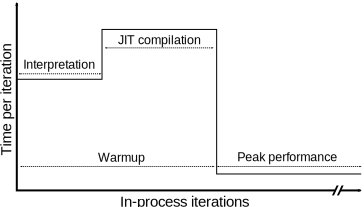
\includegraphics[width=.5\textwidth]{img/picturebook_warmup}
\caption{The traditional notion of warmup: a program starts slowly executing in
an interpreter; once hot parts of the program are identified, they are
translated by the JIT compiler to machine code; at this point warmup
is said to have completed, and peak performance reached.}
\label{fig:trad}
\end{figure}

We expected our experiment to validate Hypothesis H1, allowing us to
easily compare warmup across VMs. While some benchmarks on some VMs run as per
traditional expectations, we found a number of surprising cases. At
the most extreme, some benchmarks never warmup, staying at their initial performance
levels indefinitely and some slowdowns, getting slower over time. Even for
those benchmarks that appear to warmup in a traditional fashion, there are
various performance patterns that make presenting a simple performance number
difficult. Of the eight VMs we looked at,
none consistently warmed under the traditional model \edd{check this is true
when we have all the results}.

Our results thus suggest that the traditional view of warmup is badly out of
date---if it ever held at all. We suggest it is better to think of most benchmarks as
generally converging on a \emph{steady state} of performance (be that faster or
slower than initial execution). When a benchmark does not converge on a steady
state, we suggest that it is impossible to give meaningful performance figures.
We believe our results are of interest to VM writers, but also to users of
those VMs. Authors may not have considered the different types of warmup
behaviour (or found benchmarks which trigger such behaviour), whereas users may
obtain a greater understanding of why their programs do not perform as well as
they had expected.

%This paper's contributions are as follows:
%\begin{enumerate*}
%  \item \laurie{blah blah}
%\end{enumerate*}
%
%This paper's structure is as follows. \laurie{blah blah}


\section{Background}
\label{sec:warmup}

When a program begins running on a JIT compiled VM, it is typically (slowly)
interpreted; once `hot' (i.e.~frequently executed) loops or methods are
identified, they are dynamically compiled into machine code; and subsequent
execution of those loops or methods uses (fast) machine code rather than the
(slow) interpreter. Once machine code generation has completed, the VM is
traditionally said to have finished warming up, and the program to be executing
at peak performance.\footnote{This traditional notion applies equally to VMs
that perform immediate compilation instead of using an interpreter, and to
those VMs which have more than one layer of JIT compilation (later JIT
compilation is used for `very hot' portions of a program, and tolerates slower
compilation time for better machine code generation).}

Figure~\ref{fig:trad} shows the expected performance profile of a
program subject to the conventional model of warmup. Exactly how long warmup
takes is highly dependent on
the program and the JIT compiler, but this basic assumption about the
performance model is shared by every JIT compiling
VM~\cite{kalibera13rigorous}.

Benchmarking of JIT compiled VMs typically focusses on peak
performance.\footnote{There are various cultural and technical reasons for this,
ranging from the difficulty of determining warmup, to the flattering effect that
peak performance can imbue on programs that are JIT compiled.} The
methodologies used are typically crude: benchmarks are run for a number
of in-process iterations within a single VM process execution
The first $n$ in-process iterations are then discarded, on the basis that warmup
will have completed at some point before $n$. It is common for
$n$ to be a hard-coded number -- in our experience, it is often set at 5 -- used
for all benchmarks.

One of the obvious flaws in this simple methodology is that one does not know if warmup
has completed by in-process iteration $n$. A more sophisticated VM benchmarking methodology
was developed by \kalibera to solve a number of issues when benchmarking JIT
compiling VMs~\cite{kalibera12quantifying,kalibera13rigorous}. The basic idea is
that, for a given VM / benchmark combination, a human must inspect the data from
executing a small number of VM process executions, and determine at which in-process iteration the
benchmark has definitively warmed up. A larger number of VM process executions are then
run, and the previously determined cut-off point applied to each process's
iterations. The \kalibera methodology observes that some benchmarks do not
obviously warmup; and that others follow cyclic patterns post-warmup
(e.g.~in-process iteration $m$ is slow, $m+1$ is fast, for all even values of $m > n$). In
the latter case, the \kalibera methodology requires a consistent in-process iteration in
the cycle to be picked for all process executions, and that used for statistical analysis.

To the best of our knowledge, the \kalibera methodology is the most
sophisticated currently available (see its use in
e.g.~\cite{barrett15approaches,grimmer15dynamically}). While the \kalibera
methodology is a real improvement over crude benchmarking methodologies,
our experience has been that there remain cases where it remains hard to produce
satisfying benchmarking statistics. Crucially, the methodology does not
provide a firm way of determining when warmup has completed. Because of this
``determining when a system has warmed up, or even providing a
rigorous definition of the term, is an open research problem''~\cite{seaton15phd}.


\section{Methodology}
\label{sec:methodology}

To test Hypothesis H1, we designed an experiment which uses a suite of
micro-benchmarks: each is run with 2000 in-process iterations and repeated
using 10 process executions. In order
that we the data we obtain high-quality data, we have carefully designed our
experiment to be repeatable and to control as many potentially confounding variables as
is practical.

In this section we detail our methodology: the benchmarks we use and the
modifications we made to them; the machines we used for benchmarking; the VMs we
benchmarked; and the \krun system we developed to run benchmarks.


\subsection{The Micro-benchmarks}

The micro-benchmarks we use are as follows: \binarytrees, \spectralnorm, \nbody,
\fasta, and \fannkuch from the Computer Language Benchmarks Game (CLBG); and
\richards. For each benchmark, we provide C, Java, Javascript, Python, Lua, PHP,
and Ruby versions.\footnote{Our need to have implementations in a wide variety
of languages restricted the micro-benchmarks we could use.} Since most of these
benchmarks have multiple implementations in any given language, we picked
the same versions used in~\cite{bolz14impact}, which represented the fastest
performers at the point of that publication.

Readers can be forgiven for initial scepticism about this set of micro-benchmarks.
They are small and widely
used by VM authors as optimisation targets. In general they are more effectively
optimised by VMs than average programs; when used as a proxy for other types
of programs (e.g.~large programs), they tend to overstate the effectiveness of
VM optimisations. In our context, this weakness is in fact a strength: we need
small, deterministic, and widely examined programs so that we can test
Hypothesis \hypone. Put another way, if we were to run arbitrary programs
and find unusual warmup behaviour, a VM author might reasonably counter that
``you have found the one program that exhibits unusual warmup behaviour''.

For the avoidance of doubt -- and in
contrast to some other experiments we are aware of -- we
did not interfere with any VM's Garbage Collection (GC) (e.g.~we did not
force a collection after each iteration).


\subsubsection{Ensuring Determinism}

We wish to ensure, as far as possible, that the micro-benchmarks are
deterministic from the user's perspective, by which we mean that they
take precisely the same path through the Control Flow Graph (CFG) on each
execution and iteration. Note that this definition deliberately focuses
on non-determinism that is controllable by the user; other forms of
non-determinism within the VM are deliberately excluded, as they are
part of what we are trying to measure (e.g.~objects in memory may be allocated
or garbage collected non-deterministically). To test this, we created variants
of all benchmarks with \texttt{print} statements at all possible points of
divergence (e.g.~\texttt{if} statements' true and false branches).\footnote{These
variants are available in our experimental suite.}

We first ran the benchmarks many \edd{how many?} times, and compared the outputs
of different runs. This showed that the \fasta benchmark was non-deterministic
in all language variants. This is because \fasta generates random numbers with
a seed that is initialised only at the very start of the benchmark, thus
causing each in-process iteration to generate different random numbers. We
fixed this simply by moving the random seed initialisation to the start
of the in-process iteration main loop.

Bearing in mind surprising
results such as the importance of link order~\cite{mytkowicz09surprising}, we
then used two different machines to compile VMs and then ran the benchmarks
on these machines.

For the Java benchmarks we made sure that the benchmark classes are loaded
before the first iteration of the benchmarks. Otherwise, the first iteration
is often dominated by the time the class loading takes, which is not what we
are interested in measuring.


\subsection{Measuring Computation and Not File Performance}

Micro-benchmarks perform computation which is not then used. Highly optimising
compilers notice this, and can often optimise away part or all of a
micro-benchmark's computation. To avoid this happening, most micro-benchmarks
output intermediate and final results to \texttt{stdout} so that computation is
not optimised away. However, one can quickly end up in a situation where one is
unintentionally measuring, in part or whole, the performance of file routines in
the OS libraries and the kernel.

To lessen the possibility of optimising compilers removing benchmark computation,
we modified all of the benchmarks to calculate a checksum on each in-process iteration.
At the end of each iteration, the checksum is validated against an expected
value and the value printed out if the check fails. By writing benchmarks in
this style, we make it difficult for optimising compilers to remove the
main bulk of the benchmark. Note that each micro-benchmark has a single checksum value for all
language variants, which also provides some assurance that each language variant is
performing the same work.


\subsection{Benchmarking Machines}

%We used three machines and two operating systems:
We used two machines:
\begin{description*}
  \item[\bencherthree] A quad-core i7-4790K 4GHz machine with 24GB of RAM, running Debian 8.
  \item[\bencherfive] A quad-core i7-4790 3.6GHz machine with 32GB of RAM, running Debian 8.
%  \item[\benchersix] Identical hardware to \bencherfive, but running OpenBSD 5.8.
\end{description*}
These machines allow us to investigate the effects of moderately different
hardware (\bencherthree and \bencherfive run the same operating system with the
same updates installed)
%as well as moderately different operating systems
%(\bencherfive and \benchersix have almost identical hardware, but run different
%Unix
%variants). With regards to hardware and operating systems, we started with the
%following hypothesis:
%\begin{description}
%  \item[\hyptwo] Moderately different hardware and operating systems have little effect on warmup patterns.
%\end{description}
%We deliberately use the word `moderately', since significant changes of hardware
%(e.g.~x86 vs.~ARM) or operating system (e.g.~Linux vs.~Windows) implies that
%significantly different parts of the VMs will be used (e.g.~different machine
%code backends may be of differing levels of maturity).

We disabled turbo boost and hyper-threading in the BIOS. Turbo boost is a
feature which allows CPUs to temporarily run in an extremely high-performance
mode; this eventually causes the CPU to exceed its safe thermal limit, and
performance is then reduced to a lower limit. Turbo boost can thus cause long-running processes to
appear to suddenly slow down. Hyper-threading gives the illusion that a single
physical core is in fact more than one core, allowing more programs to
run semi-simultaneously. However, hyper-threading causes programs to interfere
with each others in complex ways, introducing considerable noise. It
is of no real benefit in our situation, where we do not make use all of the
physical cores in our benchmarking machines.


\subsection{VMs under investigation}

We ran the benchmarks on the following language implementations:
\begin{description*}
\item[GCC] Version 4.9.2 from Debian packages
\item[Graal \#9dafd1dc5ff9] Oracle's next-gen VM targeting Java.
\item[HHVM 3.7.1] Facebook's PHP JIT.
\item[JRuby/Truffle \#7f4cd59cdd1c8] A Ruby interpreter using Graal for dynamic compilation.
\item[HotSpot 8u45b14] The most widely used Java VM.
\item[LuaJIT 2.0.4] A tracing JIT for Lua.
\item[PyPy 4.0.0] A meta-tracing VM for Python-2.7.
\item[V8 4.8.271.9] Google's JIT for Javascript.
\end{description*}
\edd[final]{Add to list: CPython 2.7.10, The reference Python implementation}%
Although not a VM, GCC serves as a baseline to compare the VMs against.

We created a build script which downloads, configures, and builds fixed
versions of the
VMs, ensuring we can easily repeat builds.
All VMs were compiled with GCC/G++ 4.9.2.\edd[final]{Say something about a
fixed GCC accross platforms}\edd[final]{Neither HHVM nor
JRuby/Truffle has currently been ported to OpenBSD, and thus we were unable to
run those VMs on OpenBSD.}


\subsection{\krun}

We developed a tool called \krun to fully automate the running of benchmarks
and to control the environment under which the benchmarks run. \krun itself is a
`supervisor' process which first configures a system before running VM-specific
benchmarks, monitoring the system for any signs of errors during benchmarking,
and writing results to a compressed JSON file. \krun is invoked with a
configuration file which describes the VMs, benchmarks, and number of process
executions and in-process iterations to
be executed. \krun is a generic tool, with utility beyond this paper, though
here we discuss only the parts relevant to this paper's experiment.

In the rest
of this subsection, we describe: the variables which \krun controls, both
platform neutrally and platform specific; and how it collects iterations data.
Note that, although \krun has modes in which various checks are disabled, we
describe only the `full run' mode in which such checks are enforced.


\subsubsection{Platform Independent Controls}

Several of \krun's operations work on all supported platforms. \krun imposes a
consistent heap (we set 2GiB) and stack (we set 8MiB) \texttt{ulimit} for each
VM (we used a 2GiB heap and a 8MB stack).\footnote{Note that Linux allows users
to inspect these values, but to allocate memory beyond them.} Benchmarks are run
as a specific Unix user `\texttt{krun}' with a fresh environment. When run in
`production' mode, \krun reboots the system before each benchmark (including
before the first benchmark) to ensure that the system is in a known state
(e.g.~if a benchmark caused a system to transfer memory to disk-based swap,
rebooting ensures that later benchmarks are not affected). After reboot, \krun
is run from \texttt{/etc/rc.local}; it pauses for 3 minutes to allow the system
to fully initialise before running the next benchmark.

\krun performs two types of monitoring before and during benchmark execution.

First, \krun monitors the system's \texttt{dmesg} buffer, informing the user of
any changes. We implemented this feature after noticing that one of the
machines we had earlier ear-marked for running benchmarks occasionally
overheated, leaving only a single line in the \texttt{dmesg} to inform us that
performance was throttled; as
readers will no doubt hope, we did not use this machine for our final
benchmarking.

Second, \krun monitors the system temperature. Since modern systems downgrade
their performance when they get too hot, \krun ensures that all benchmarks
start with the system temperature at (approximately) the same target. When
initially invoked, \krun collects temperature readings from all available
temperature sensors. Before running
further benchmarks, it then waits for the CPU to cool down to within 10\%{} of
the starting temperatures. If the system fails to cool down to within
this threshold in 10 minutes, \krun terminates the entire experiment. Note that
since \krun has no way of knowing what a `cool' temperature is in advance,
\krun is forced to assume that the machine is adequately cool when first invoked.


\subsubsection{Linux-specific Controls}

On Linux, \krun enables several additional factors to be controlled.

\krun sets the CPU frequency to the highest possible non-over-clocked value
(without over-clocking). The user must first disable Intel P-state support in
the kernel by passing the kernel argument \texttt{intel\_pstate=disable}.
\krun verifies P-states are disabled and uses \texttt{cpufreq-set} to set
the CPU governor to \texttt{performance} mode. See
Section~\ref{sec:threats} for more discussion on Intel P-states.

\krun checks that it is running on a `tickless' kernel. By default, the Linux kernel
queries each CPU \laurie{1000 times per sec by default I think?} to
determine which processes are active; this querying interferes with running
processes; a tickless kernel eliminates most \laurie{or `all'?}\edd{I'm not
sure. I'm not even sure how much impact ticks impose. We are using a tickless
kernel as a precaution more than anything else.}\laurie{what we learnt from the isolcpus thing is that if we don't understand the effect of a setting, we shouldn't fiddle with it. so let's work out what the effect is. in this case, it shouldn't be hard to find documentation about what the difference is} of this effect.

Linux's \texttt{perf} system dynamically profiles system performance by
repeatedly sampling hardware counters. We became aware of \texttt{perf} when
\krun's \texttt{dmesg} checks notified us that the kernel had decreased the
sample-rate as it determined that it was sampling too often. Since \texttt{perf}
can interrupt benchmarking, its existence is undesirable, particularly since its
effects can vary over time. Although \texttt{perf} cannot be disabled entirely,
\krun sets the sample-rate to the smallest possible value of 1 sample per
second.

Finally, \krun disables Address Space Layout Randomisation (ASLR). While this is
a sensible security precaution for everyday use, it makes it difficult to
compare the performance of even a single binary.\footnote{The Stabilizer
system~\cite{curtsinger} is an intriguing approach for obtaining reliable
statistics in the face of features such as ASLR. Unfortunately we were not able
to build it on a modern Linux system.} \krun sets the
\texttt{randomize\_va\_space} entry in \texttt{/proc} to 0, disabling ASLR
globally.


%\subsubsection{OpenBSD-specific Controls}
%
%Relative to Linux, OpenBSD exposes many fewer knobs to users. Nevertheless,
%there are two OpenBSD specific features in \krun.
%
%First, \krun sets CPU performance to maximum by invoking \texttt{apm -H} prior
%to running benchmarks. This is equivalent to setting Linux's CPU governor to
%\texttt{performance} mode, but note that OpenBSD offers no means of changing
%Intel P-states.
%
%Second, \krun sets OpenBSD's default \texttt{malloc} implementation to be
%deterministic. By default, OpenBSD's \texttt{malloc} performs several operations
%for security purposes, including allocating guard pages and randomising layout.
%We set the \texttt{MALLOC\_OPTIONS} environment variable to \texttt{sfghjpru},
%turning it into a more traditional, and hopefully largely deterministic,
%\texttt{malloc}.


\subsubsection{The Iterations Runners}

Since we run benchmarks in several different languages, we need a way to report
timings from benchmarks to \krun. For each language, we created an
\emph{in-process iterations runner}. When \krun wants to run a benchmark, it executes the
appropriate in-process iterations runner for that language, passing it the name of the
benchmark to be run, and the desired number of in-process iterations. The in-process iterations runner
then dynamically loads the benchmark, and repeatedly executes the main body of
the benchmark. The in-process iterations runner calls a monotonic timer with
sub-millisecond accuracy before and after each iteration, recording the result
into a list; when the iterations are complete, it returns the results
to \krun by printing a JSON list to stdout.

Most VMs and languages expose access to the low-level monotonic timing
\texttt{clock\_gettime} function as standard. We extended V8, HHVM and JRuby/Truffle
to expose this monotonic clock via a user-visible function.
%On OpenBSD, we use
%the \texttt{CLOCK\_MONOTONIC} timer; on Linux this timer is subject to
%interference from the \texttt{adjtime} function, and we thus use the
%\texttt{CLOCK\_MONOTONIC\_RAW} timer.


\section{Results}
\label{sec:Results}

After running all benchmarks as described we analysed the benchmarks in a
two-step process. In the first step we visually inspected the run sequence
graphs of all the benchmark executions, per benchmark and virtual machine. In
doing so we noted whether the virtual machine followed the expected warmup
behaviour for this benchmark as described in Section~\ref{sec:warmup}. This was
the case of \cfbolz{add numbers} X out of Y benchmarks. In a second step we
identified groups of ``anomalies'', i.e. repeating ways of how benchmark
executions deviated from the expected warmup behaviour, which we describe in a
qualitative way. In the following we will
present the run-sequence diagrams of benchmarks that have expected warmup
behaviour, as well descriptions and examples for all the anomalies.

\cfbolz{need some examples of nice benchs}


\subsection{Outliers}
\label{sub:outliers}

Outliers are iterations of a benchmark that take significantly longer than the
other iterations, even taking the randomness of the benchmark iterations into
account.

Figure~\ref{fig:examples:outliers1} shows one such example, which includes an
outlier around iteration $900$ that runs more than $0.5s$ slower than the
measurements either side of it.

\begin{figure}[h!]
\centering
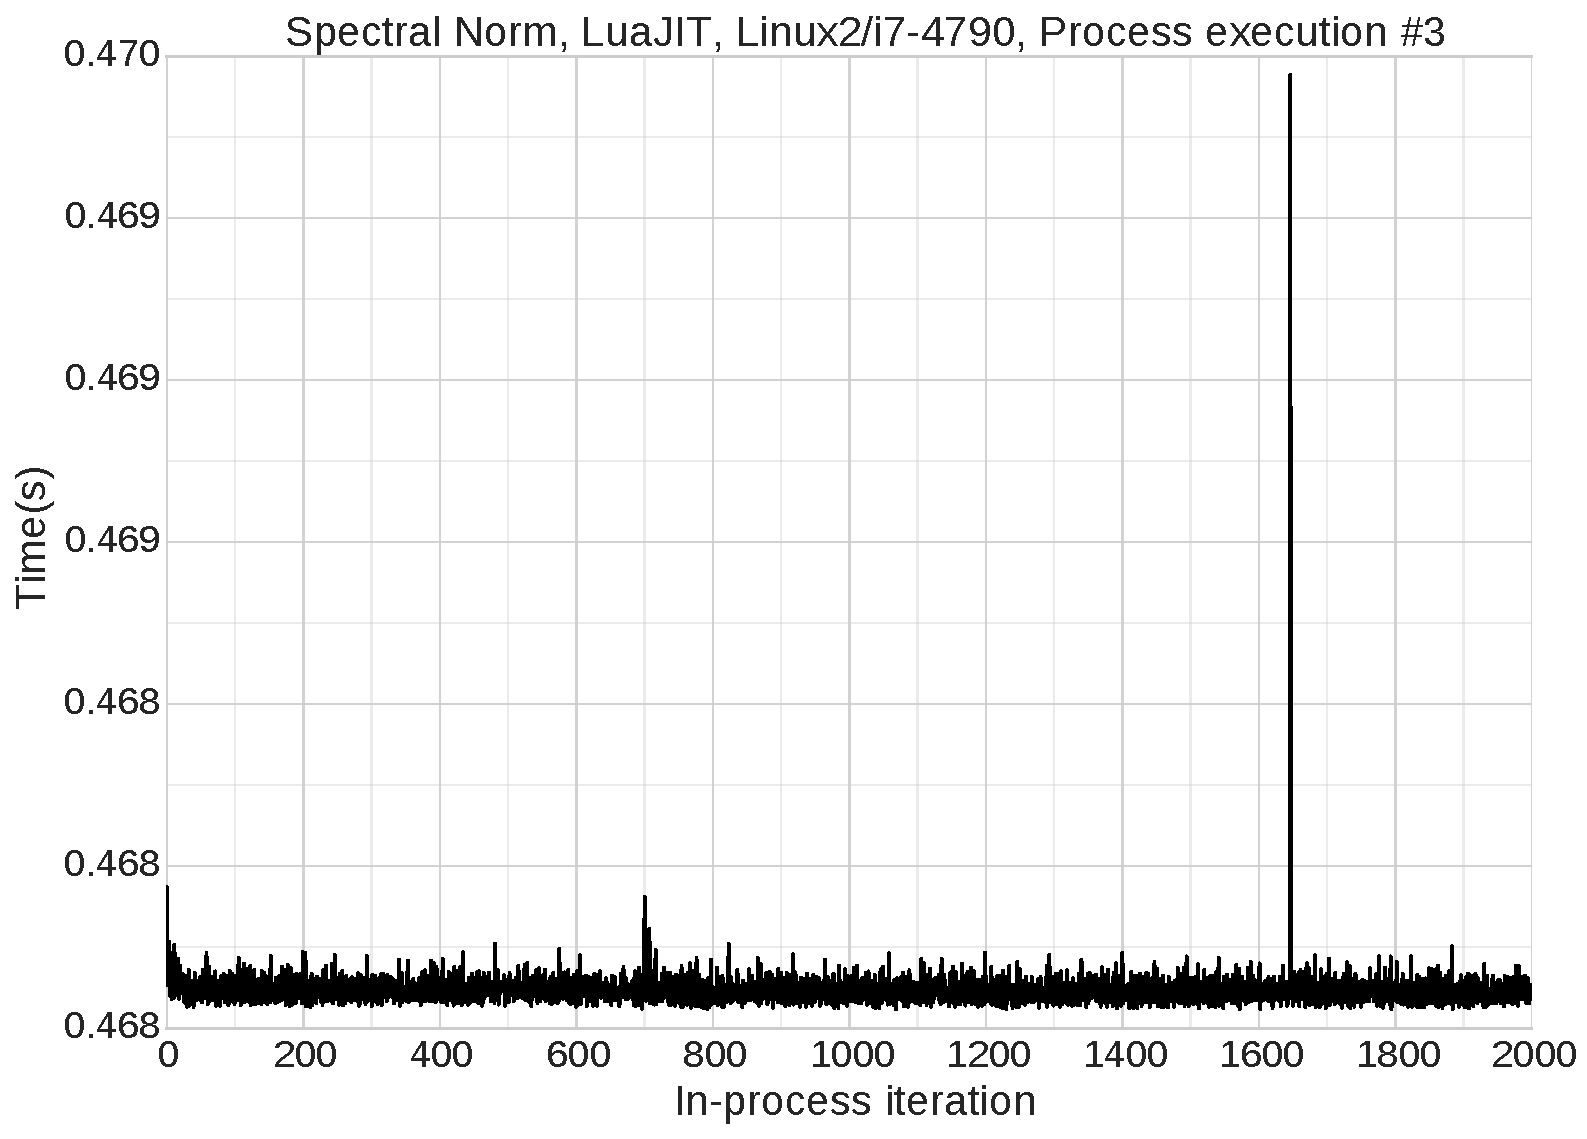
\includegraphics[width=.46\textwidth]{examples/outliers1}
\caption{Example of a benchmark with outliers.}
\label{fig:examples:outliers1}
\end{figure}


\subsection{Slowdowns}
\label{sub:slowdowns}

\sarah[final]{This is one area were the sliding-window average might be useful (i.e. in detecting a slow-down).
One possible way forward would be to find a technique for performing hypothesis testing on time-series data, then running tests to determine whether the sliding-mean in one part of the chart is significantly different to the sliding-mean in an earlier phase of the execution.
This technique would also help to determine precisely when the warm-up phase is over and the JIT has kicked in.}

A few benchmarks exhibit slow downs, where the first few iterations of a
benchmarks are faster than the eventual mean after ``warm up''.

Figure~\ref{fig:examples:slowdown1} shows one such example.

\begin{figure}[h!]
\centering
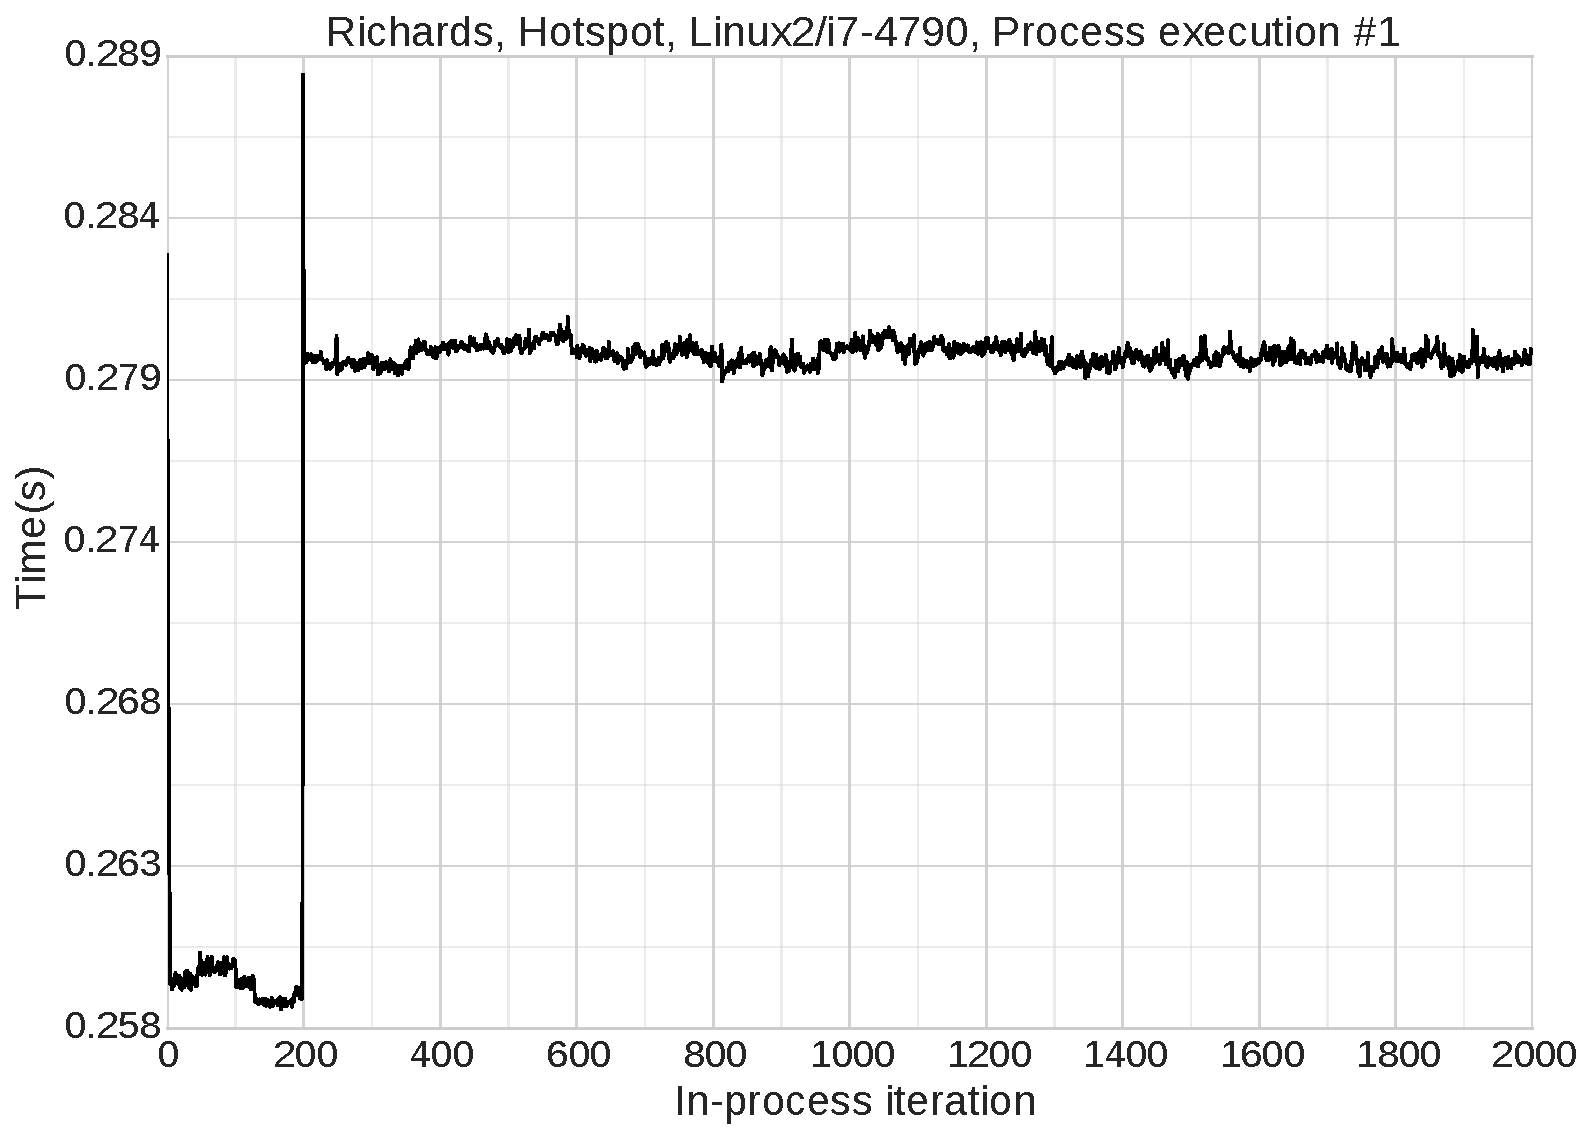
\includegraphics[width=.46\textwidth]{examples/slowdown1}
\caption{Example of a benchmark with a slowdown.}
\label{fig:examples:slowdown1}
\end{figure}



\subsection{Cyclic Behaviour}
\label{sub:cyclic}

Cyclic behaviour occurs in a number of benchmarks, which is a pattern of $n$
iterations that have similar timing results and keeps repeating across the
benchmark runs.

Figure~\ref{fig:examples:cycles1} shows one such example.

\begin{figure}[h!]
\centering
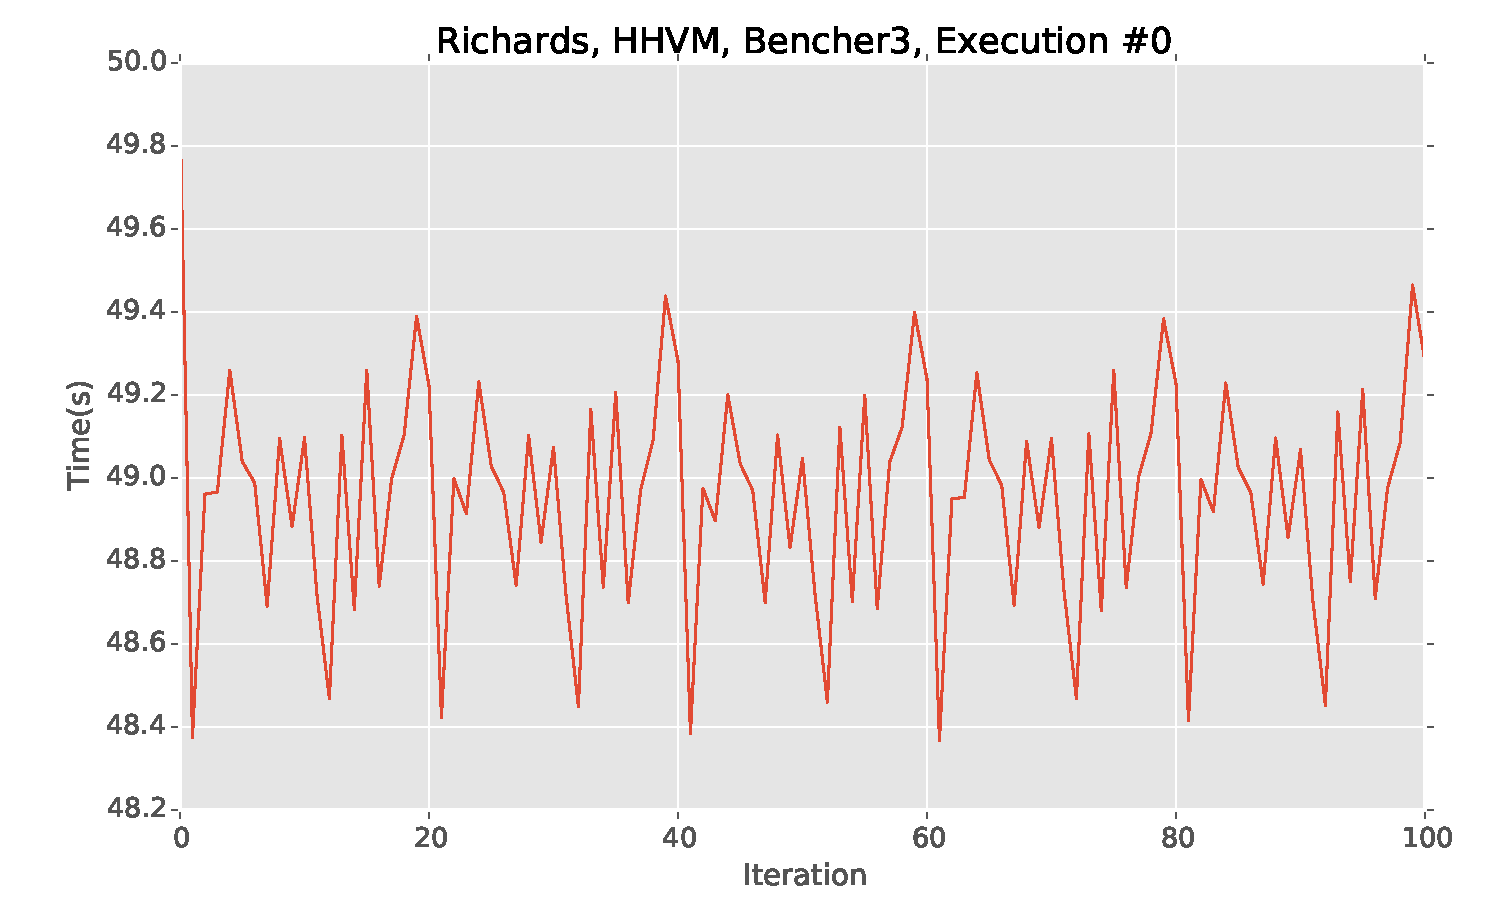
\includegraphics[width=.46\textwidth]{examples/cycles1}
\caption{Example of a benchmark with cycles.}
\label{fig:examples:cycles1}
\end{figure}


\subsection{Late Phase Changes}
\label{sub:phase}

Late phase changes occur in benchmarks where after many iterations the benchmark
changes behaviour, either by getting slower or faster, or by producing a
different pattern of randomness.

Figure~\ref{fig:examples:late1} shows one such example.

\begin{figure}[h!]
\centering
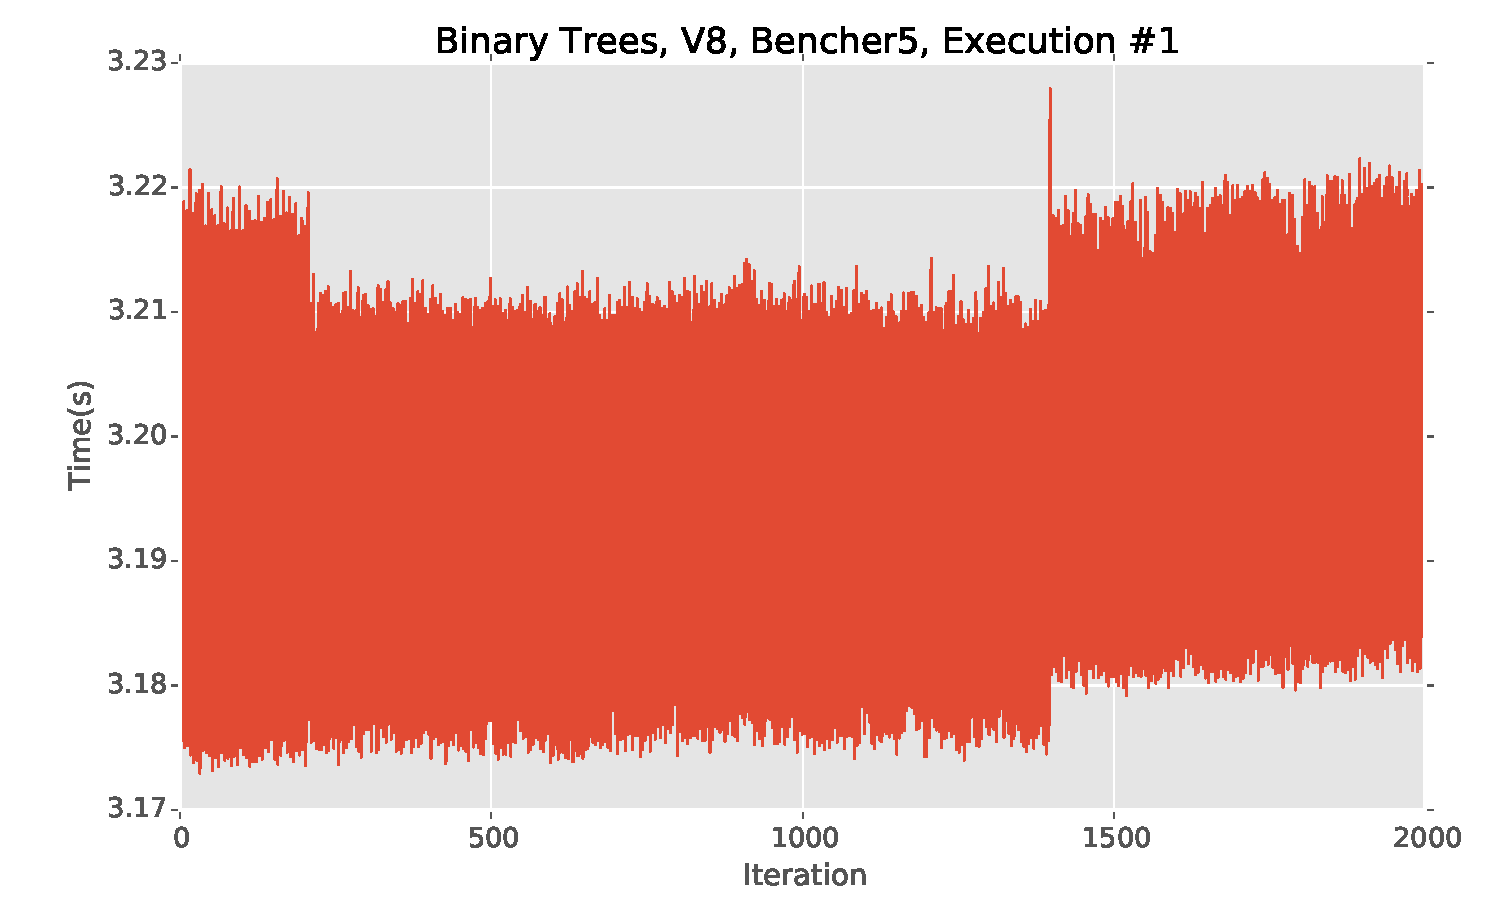
\includegraphics[width=.46\textwidth]{examples/late1}
\caption{Example of a benchmark with late phase changes.}
\label{fig:examples:late1}
\end{figure}


\subsection{Unexpectedly Long Warmup}
\label{sub:long}

The common understanding of warmup behaviour usually assumes that for such
small programs warmup is done after a few iterations. However, there are
benchmarks where performance improves after many hundred iterations.

\begin{figure}[h!]
\centering
\cfbolz{we need an example here}
\caption{Example of a benchmark with unexpectedly long warmup.}
\label{fig:examples:long}
\end{figure}

\subsection{Inconsistent Effects}
\label{sub:inconsistent}

A number of benchmarks have wildly different behaviour between different
iterations on the same machine, or between iterations of different machines.

Figure~\ref{fig:examples:consistent_weirdness1} shows a case where
unexpected behaviours are consistent between machines and executions.
Figure~\label{fig:examples:inconsistent_weirdness1} shows an example where
effects differ between both machines and executions.

\begin{figure*}[h!]
\centering
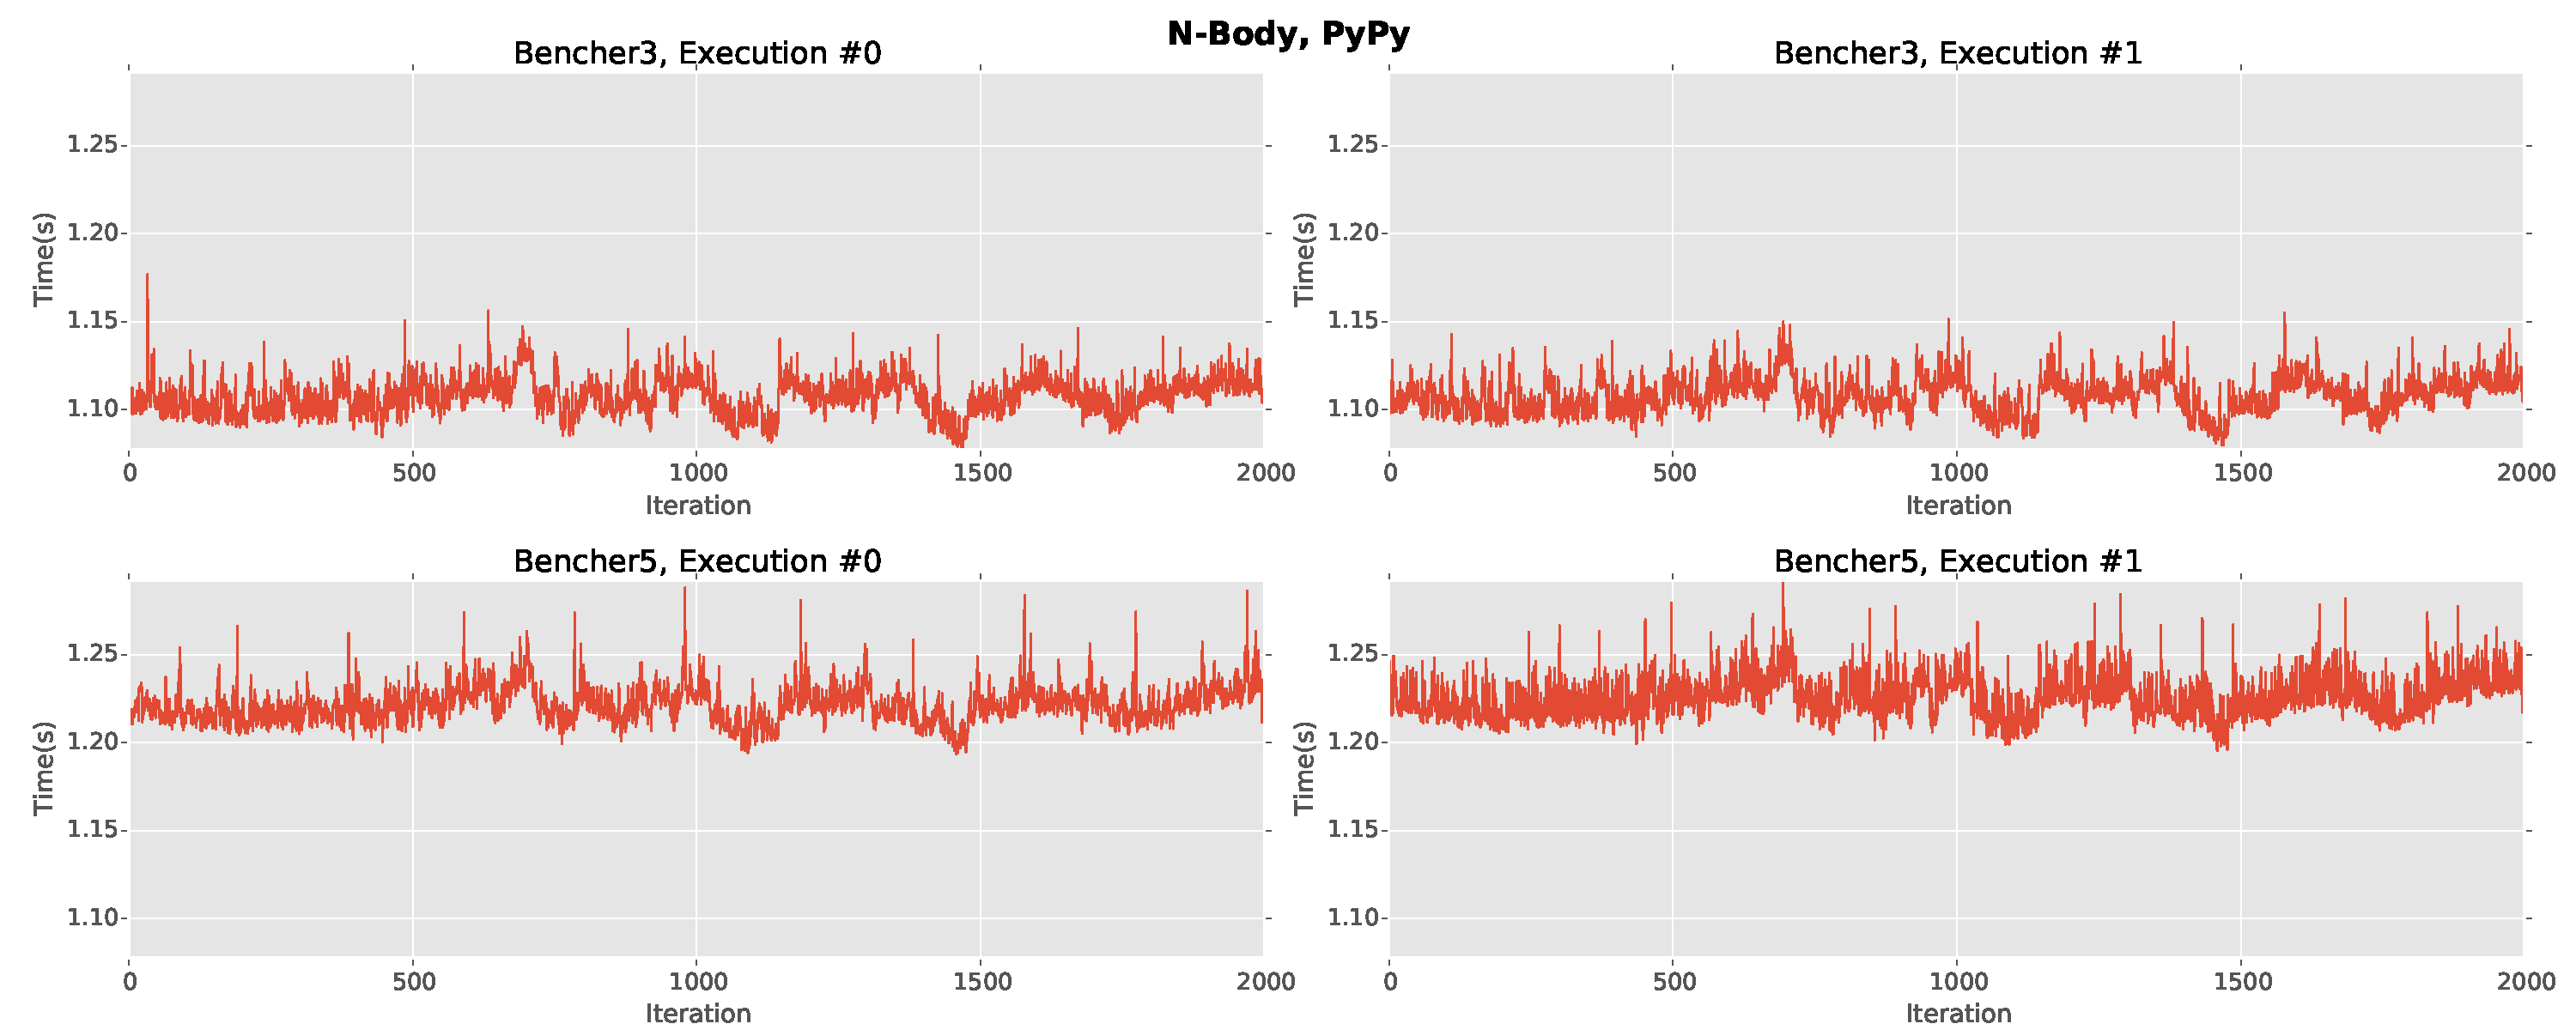
\includegraphics[width=\textwidth]{examples/consistent_weirdness1}
\caption{Example of a benchmark whose effects are consistent between machines and executions.}
\label{fig:examples:consistent_weirdness1}
\end{figure*}

\begin{figure*}[h!]
\centering
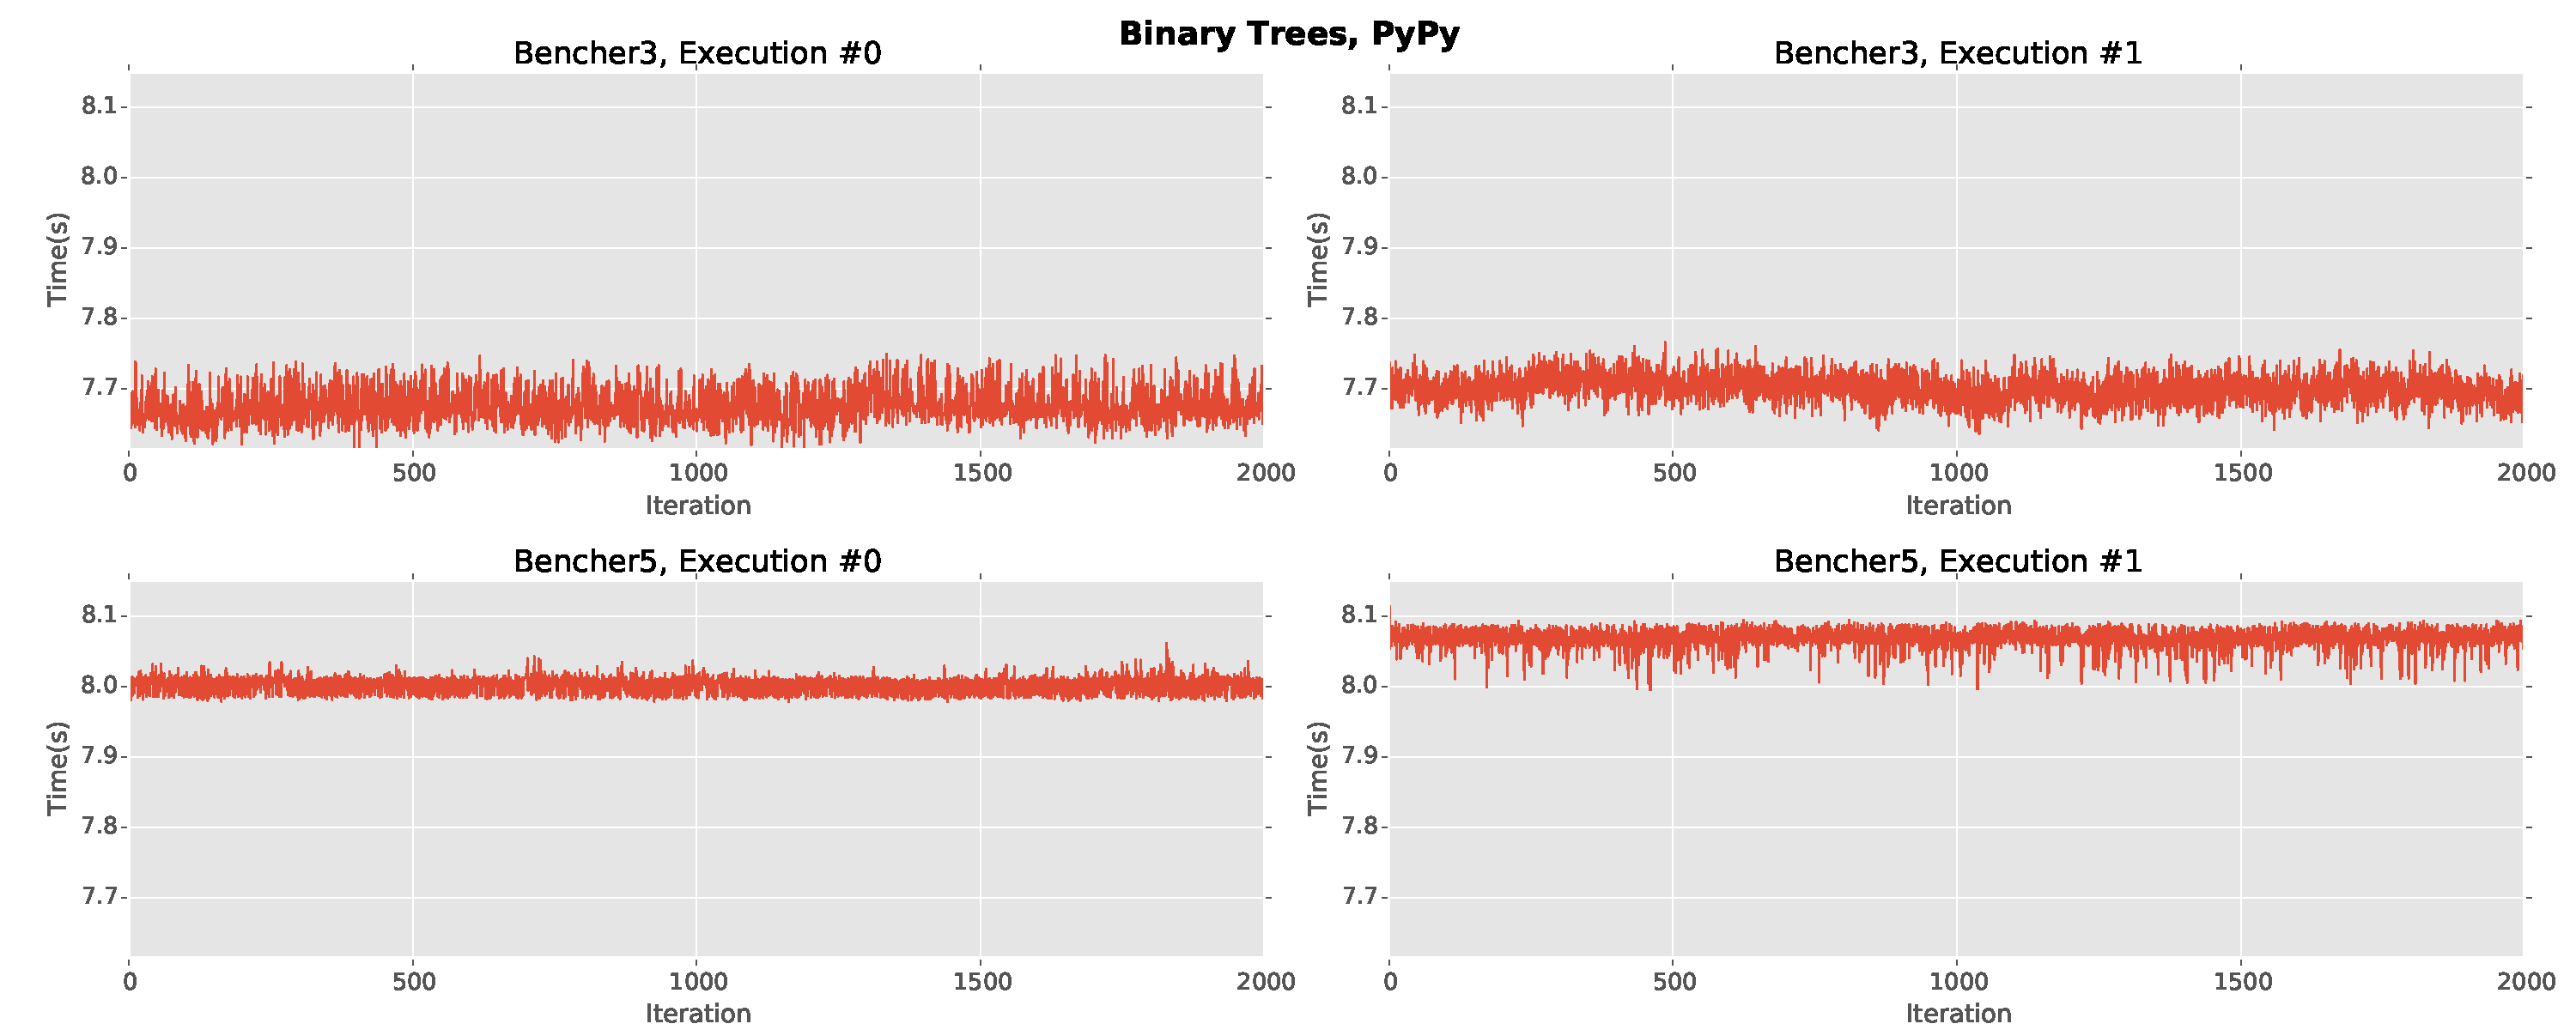
\includegraphics[width=\textwidth]{examples/inconsistent_weirdness1}
\caption{Example of a benchmark whose effects are inconsistent between machines and executions.}
\label{fig:examples:inconsistent_weirdness1}
\end{figure*}


\section{Threats to Validity}
\label{sec:threats}

While we have designed our experiment as carefully as possible, we do not
pretend to have controlled every possibly confounding variable. Indeed, our
experience when designing the experiment has been one of gradually uncovering
confounding variables whose existence we had not previously imagined. It
is all but guaranteed that there are further confounding variables that we
do not know about; some of these may be controllable, although many may not be.
It is possible that currently unknown confounding variables have coloured all
our results.

We have tried to gain a partial understanding of the effects of different
hardware on benchmarks by using benchmarking machines with different hardware
(both of which run the same OS). However, while the hardware between the two is
different, much more distinct hardware is available. Greater differences in
hardware (e.g.~using a non-x86 architecture) may give different results.
However, the greater the differences in hardware, the more likely the JIT
compilers are to use different code paths (e.g.~different code generators and
the like). Put another way, an apples-to-apples comparison across very different
hardware is likely to be impossible, because the software being run will
change its behaviour.

We have not yet systematically tested whether rebuilding VMs effects warmup, an
effect noted by \kalibera. Our previous experience of JIT compilers suggests
that there is little effect in rebuilding such VMs when measuring peak
performance~\cite{barrett15approaches}. However, since measuring warm-up largely
involves measuring code that was not created by a JIT compiler, it is possible
that these effects may impact upon our experiment. To a very limited extent, the
rebuilding of VMs that occurred on our different VMs gives some small evidence
as to this effect, but this effect requires deeper investigation.

The checksums we added ensure that, at a user-visible level, each benchmark
performs equivalent work in each language variant. However, it is impossible to
say whether each performs equivalent work at the lowest level or not. For
example, choosing to use a different datatype in a language's core library may
substantially impact performance. There is also the perennial problem as to the
degree to which an individual language benchmark should maintain the structure
of other language's implementations: a benchmark for a given language could be
rewritten in a way that betters either or both of its warmup and peak
performance. From our perspective, this possibility is somewhat less important,
since we are more interested in the warmup patterns of reasonable programs,
whether they be the fastest possible or not. It is also possible that by
inserting checksums we have created unrepresentative benchmarks, though
this complaint could arguably be directed at the unmodified benchmarks too.

Although \krun does as much to control CPU clock speed as possible, modern CPUs
do not always respect operating system requests. Even on Linux, where we control
the CPU's p-State, we can not guarantee that this fixes the CPU frequency: as
the Linux kernel states, ``the idea that frequency can be set to a single
frequency is fiction for Intel Core processors''~\cite{pstate}. In
some cases, changes the CPU makes to its performance are detected and reported
by the operating system (e.g.~performance throttling due to potential
overheating); in other cases, changes may go undetected and/or unreported.
Despite this, our benchmarks show extremely predictable performance across
different hardware, suggesting that the effect of CPU performance changes are
not significant in our case.

We have identified a number of different styles of warmup (slowdown, cyclic,
etc.). However, we do not claim to have uncovered all possible warmup styles. It
is quite possible that other patterns exist that either do not show up in our
data, or which we have not detected.


\section{Discussion}
\label{sec:Discussion}

\edd{Need to give up naive definition of warmup. Unrealistic to get rid of
these anomalies. Some of benchmarking wisdom is wrong in the presence of this
stuff.} \sarah{Need some way to model the behaviour of JITs and perform
hypothesis tests (so that people can answer questions like 'does this change in
the VM actually make the JIT faster?').}

Even though we had a reasonable amount of experience designing and implementing
experiments, the experiment in this paper took more time and effort than we
expected. In part this is because there is limited precedent for such detailed
experiments. Investigating possible confounding variables, understanding how to
control them, and implementing the necessary checks, all took time. In many
cases, we had to implement small programs or systems to understand a variables
effect (e.g.~that Linux allows a process to allocate memory beyond that
specified in the soft and hard ulimit).

In some cases, we found that seemingly reasonable settings had undesireable
effects. Most notably, we trialled running experiments on a fixed CPU core which
no other processes were allowed to run on (using Linux's \texttt{isolcpus}
feature). While this removed noise from some some VMs\edd{did it actually
remove noise? Looking at the graphs again, I don't think we can claim this.},
it slowed others down by
a factor of up to 3x. The reason for this is that pinning a process to a CPU
core also pins that processes threads to the same core. Some VMs -- such as
JRuby/Truffle -- create extra threads for compilation, GC, and the like. By
running all these threads on a single core, we removed the considerable
performance benefits of running such computation in parallel.


\section{Related work}

There are two works we are aware of which explicitly note unusual warmup
patterns. Gil et al.'s main focus is on non-determinism over execution runs on
HotSpot, and the difficulties this raise in terms of providing reliable
benchmarking numbers~\cite{gil11microbenchmark}. In this process, they report at
least one benchmark (listBubbleSort) which on some executions undergoes what we
have termed slowdowns. \kalibera note the
existence of what we have called cyclical behaviour, but require the user to
manually pick one part of the cycle for measurement~\cite{kalibera13rigorous}.


\section{Conclusions}
\label{sec:conclusion}

\bibliographystyle{plain}
\bibliography{bib}


\end{document}

